% Approximation Algorithms (1 week)

Often, it is not necessary to find the best solution to a problem, but an approximation of the best solution (i.e. a good solution) is sufficient. In addition, the algorithms for the exact solution are usually very complex and the running time plays a central role in the evaluation of an algorithm.

\begin{itemize}
    \item \textbf{Turing machine}
    \begin{itemize}
        \item To compare the complexity or difficulty of an algorithm, we need to define a model computer on which the algorithm is to run.
        \item \emph{Deterministic Turing machine:} Processes an algorithm a step at a time (normal computer)
        \item \emph{Non-Deterministic Turing machine:} Can do multiple steps at a time (fictitious computer)
    \end{itemize}
    \item \textbf{Complexity classes}
    \begin{itemize}
        \item \emph{P:} Set of decision problems that can be solved by a deterministic Turing machine in \textbf{p}olynomial time
        \item \emph{NP:} Set of decision problems that can be solved by a \textbf{n}on-deterministic Turing machine in \textbf{p}olynomial time
        \item All problems in \textbf{P} are also in \textbf{NP} (Open question: Are all problems in \textbf{NP} also in \textbf{P})
    \end{itemize}
    \item \textbf{Problem reduction}
    \begin{itemize}
        \item \emph{Reducibility:} Problem $X$ can be transformed into problem $Y$ by a reduction function such that the answers of $X$ and $Y$ are the same.
        \item If a problem $X$ can be reduced to problem $Y$, each algorithm solving $Y$ can also be used to solve $X$ (If there is a polynomial-time algorithm for problem $Y$, there is also one for $X$).
        \item e.g. Problem of taking the square of a number is polynomial-reducible to the problem of multiplying two numbers.
    \end{itemize}
    \item \textbf{NP-completeness}
    \begin{itemize}
        \item 
    \end{itemize}
\end{itemize}

Most of the problems that we want to solve with approximation algorithms are NP-complete, which is because they follow a boolean logic, are subject to the graph data type, etc. When designing an algorithm, the main goal is to find the optimal solution quickly for all possible cases. Since this is virtually impossible for an approximation, we follow these steps:

\begin{itemize}
    \item Relax requirement for \emph{speed:} If N is small, an algorithm with exponential running time might be okay.
    \item Relax requirement for \emph{generality:} Isolate important special cases that can be solved in polynomial time.
    \item Relax requirement for \emph{optimal solution:} Find near-optimal solutions (approximations) in polynomial time (either worst-case or average case) à in practice, this is often good enough
\end{itemize}

A well-known problem from the world of approximation algorithms is the \emph{Traveling Salesman Problem} (TSP), in which the optimal path in a graph (undirected, weighted dense graph) is to be found, in which each vertex is visited exactly once and one starts at the same vertex as one ends. 

\begin{center}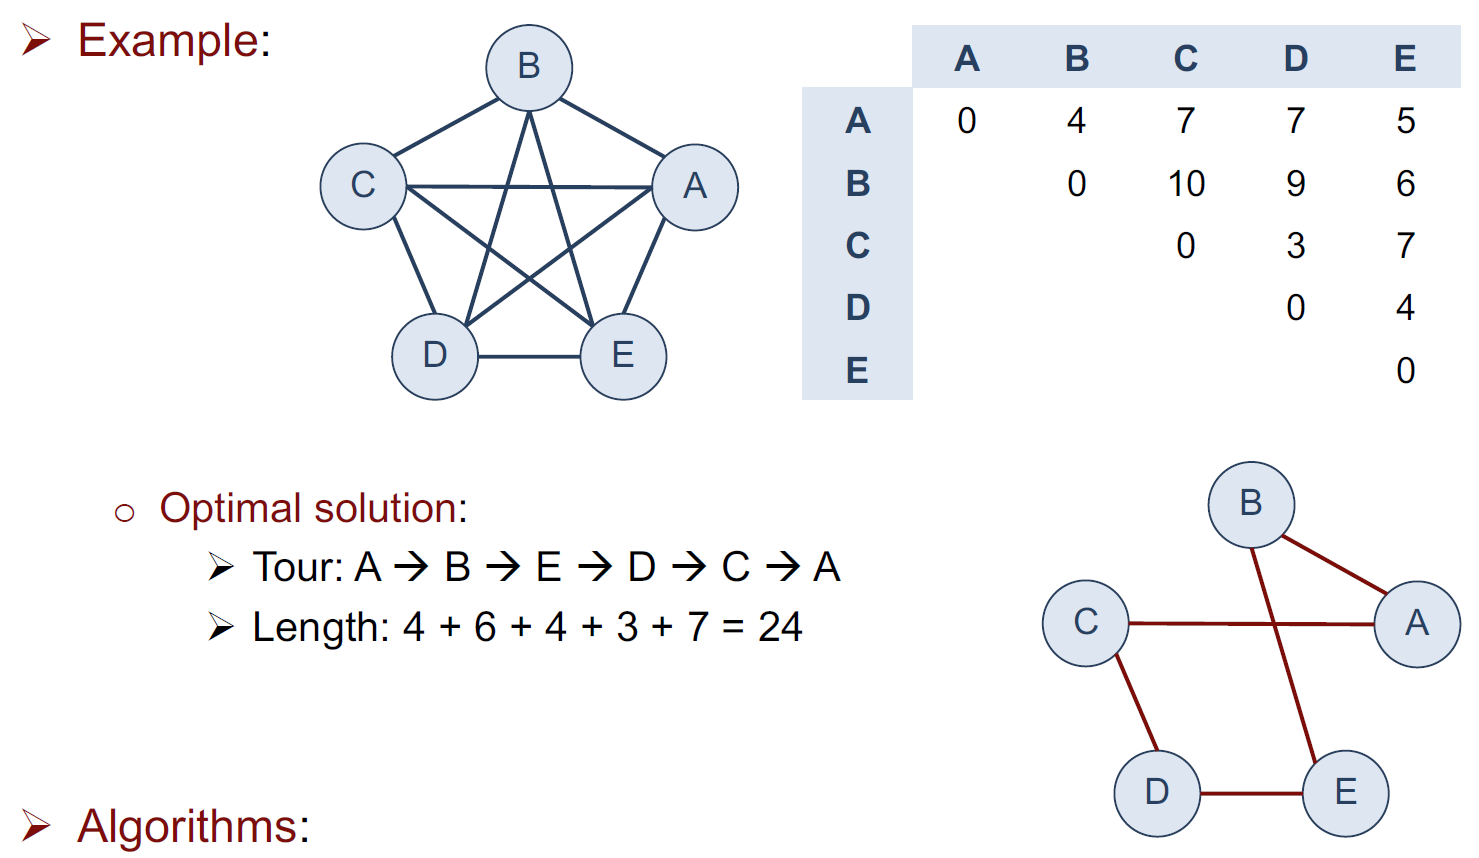
\includegraphics[width=0.85\textwidth]{img/approximation/TspOptimalSolution.png}\end{center}

It is a NP-hard optimization problem and worst-case running time is superpolynomial with $\Theta(N!)$. There are four broad types of approximation algorithms:

\begin{itemize}
    \item \textbf{Greedy Algorithm}
    \begin{itemize}
        \item At each decision point, select the option that yields the largest immediate progress towards the goal.
        \item Running time for TSP: $\Theta(N)$
    \end{itemize}
    \item \textbf{Local search}
    \begin{itemize}
        \item Guess an arbitrary solution and try to improve.
        \item Running time for TSP: difficult to estimate, but usually very efficient
    \end{itemize}
    \item \textbf{Approximate dynamic programming}
    \begin{itemize}
        \item Combine the solutions of subproblems.
        \item Running time for TSP: $\Theta(N^22^N)$
    \end{itemize}
    \item \textbf{Backtracking with heuristics}
    \begin{itemize}
        \item 
        \item Running time for TSP: difficult to estimate
    \end{itemize}
\end{itemize}

\subsection{Approximate dynamic programming}

The idea of the dynamic programming approach is to first solve subproblems of the actual problem and then combine them to find a solution. To do this, we define $S$ as the set of vertices that have not yet been visited. We start the journey at 0 and the journey ends at vertex $j\in\{1,2,\cdots,N-1\}$, where $N$ is the number of vertices. We denote the problem as $C(S,j)$ (mathematically, $C(S,j)$ is the total cost of the path), where the journey starts at 0, ends at $j$ and in between all vertices of the set $S$ without $j$ are visited. So the subproblem is to find the minimum for a vertex $i$ (penultimate vertex) that is in $S$ and is not $j$, so that we have reduced the overall problem by one vertex to $C(S-\{i\},i)$ and can raise it back to the overall problem by adding the distance $d_{i,j}$.

\begin{align}
    C(S,j)=\min_{i\in S\;i\neq j}\left\{d_{i,j}+C(S-\{i\},i)\right\}
\end{align}

Thus, we generate $N^22^N$ subproblems, each of which has a linear running time, which is why overall we have a running time of $\Theta(N^22^N)$. We want to stay at the example above We proceed as follows to implement the algorithm:

\begin{enumerate}
    \item $C(\{\},j)$ is the shortest path from $0$ to $j$, but all cities besides $j$ was already visited, so $C(\{\},j)=d_{0,j}$ is the only possible path.
    \item We first calculate all possible combinations of $C(\{S\},j)$, where only one city was not visited yet, so that $|S|=1$. Because this is a problem of we start from 0, end up $j$ and we have to visit only one city in between that, there is only one possible path for this, so we do not have to calculate an minimum.
    \begin{align*}
        C(\{1\},2)&=d_{1,2}+C(\{\},1)=d_{1,2}+d_{0,1}=14\\
        C(\{2\},1)&=d_{2,1}+C(\{\},2)=d_{2,1}+d_{0,2}=17\\
        C(\{1\},3)&=d_{1,3}+C(\{\},1)=d_{1,3}+d_{0,1}=13\\
        C(\{3\},1)&=d_{3,1}+C(\{\},3)=d_{3,1}+d_{0,3}=16\\
        C(\{1\},4)&=d_{1,4}+C(\{\},1)=d_{1,4}+d_{0,1}=10\\
        C(\{4\},1)&=d_{4,1}+C(\{\},4)=d_{4,1}+d_{0,4}=10\\
        C(\{2\},3)&=d_{2,3}+C(\{\},2)=d_{2,3}+d_{0,2}=10\\
        C(\{3\},2)&=d_{3,2}+C(\{\},3)=d_{3,2}+d_{0,3}=11\\
        C(\{2\},4)&=d_{2,4}+C(\{\},2)=d_{2,4}+d_{0,2}=14\\
        C(\{4\},2)&=d_{4,2}+C(\{\},4)=d_{4,2}+d_{0,4}=12\\
        C(\{3\},4)&=d_{3,4}+C(\{\},3)=d_{3,4}+d_{0,3}=11\\
        C(\{4\},3)&=d_{4,3}+C(\{\},4)=d_{4,3}+d_{0,4}=9
    \end{align*}
    \item Now we can increase the size of $S$ by one, so that we have $|S|=2$, but with that we have two possible values for $i$. Because of that we now have to determine a minimum between two values, but when we use the formula to reduce the problem to a smaller size of $S$, we can use the values above.
    \begin{align*}
        C(\{1,2\},3)&=\min_{i\in\{1,2\}}\left\{d_{i,3}+C(\{1,2\}-\{i\},i)\right\}\\
        &=\min\left\{\{d_{1,3}+C(\{2\},1)\},\{d_{2,3}+C(\{1\},2)\}\right\}\\
        &=\min\left\{\{9+17\},\{3+14\}\right\}=\min\{28,17\}=17\\
    \end{align*}
    \item We continue to increase the size of $S$ by one until we get to our final $S$ and fill in each step the values from before to determine the min. 
    \begin{align*}
        C(\{1,2,3\},4)&=\min_{i\in\{1,2,3\}}\left\{d_{i,4}+C(\{1,2,3\}-\{i\},i)\right\}\\
        C(\{1,2,3,4\},0)&=\min_{i\in\{1,2,3,4\}}\left\{d_{i,0}+C(\{1,2,3,4\}-\{i\},i)\right\}\\
    \end{align*}
\end{enumerate}

% finished code (but with out comments)
%\lstinputlisting[language=C++]{src/approximation/dynamic.cpp}

\subsection{Backtracking with heuristics}



% not finished code
%\lstinputlisting[language=C++]{src/approximation/backtracking.cpp}

\subsection{Greedy algorithm}

A greedy algorithm is based on always making the decision with the smallest weight from a starting point, so in terms of graph theory, that you start at a certain vertex and from there always select the edge with the smallest weight. At TSP, we proceed as follows, always keeping in mind that the result depends on the starting vertex:

\begin{enumerate}
    \item Start from a random city.
    \item Go to the nearest city not visited yet.
    \item Repeat until all cities have been visited and finally return to starting city.
\end{enumerate}

\begin{center}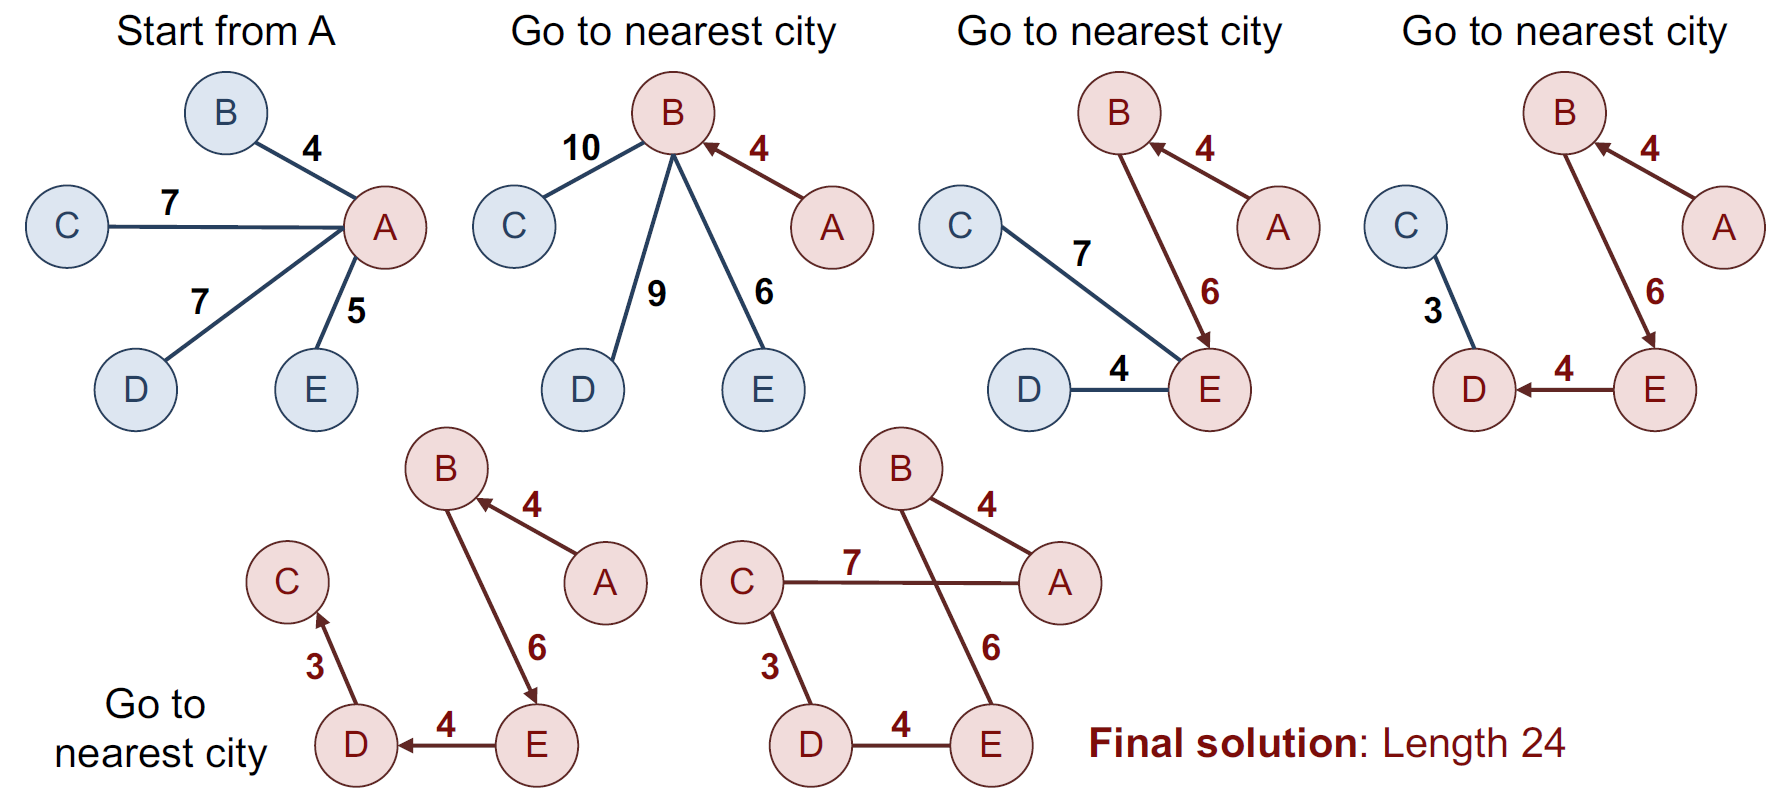
\includegraphics[width=0.85\textwidth]{img/approximation/TspGreedy1.png}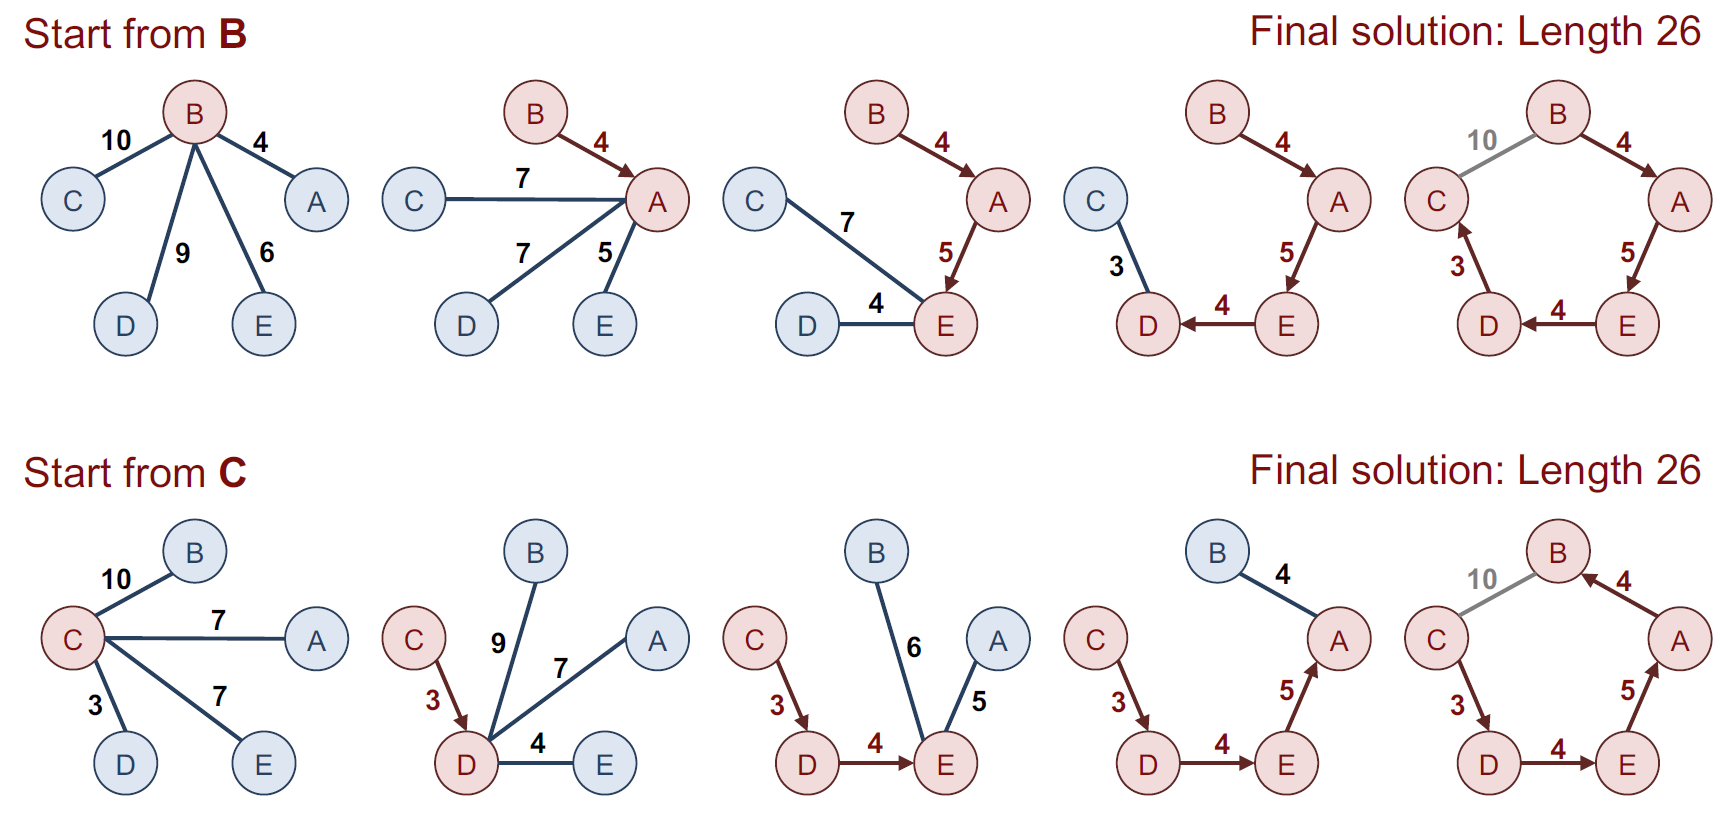
\includegraphics[width=0.85\textwidth]{img/approximation/TspGreedy2.png}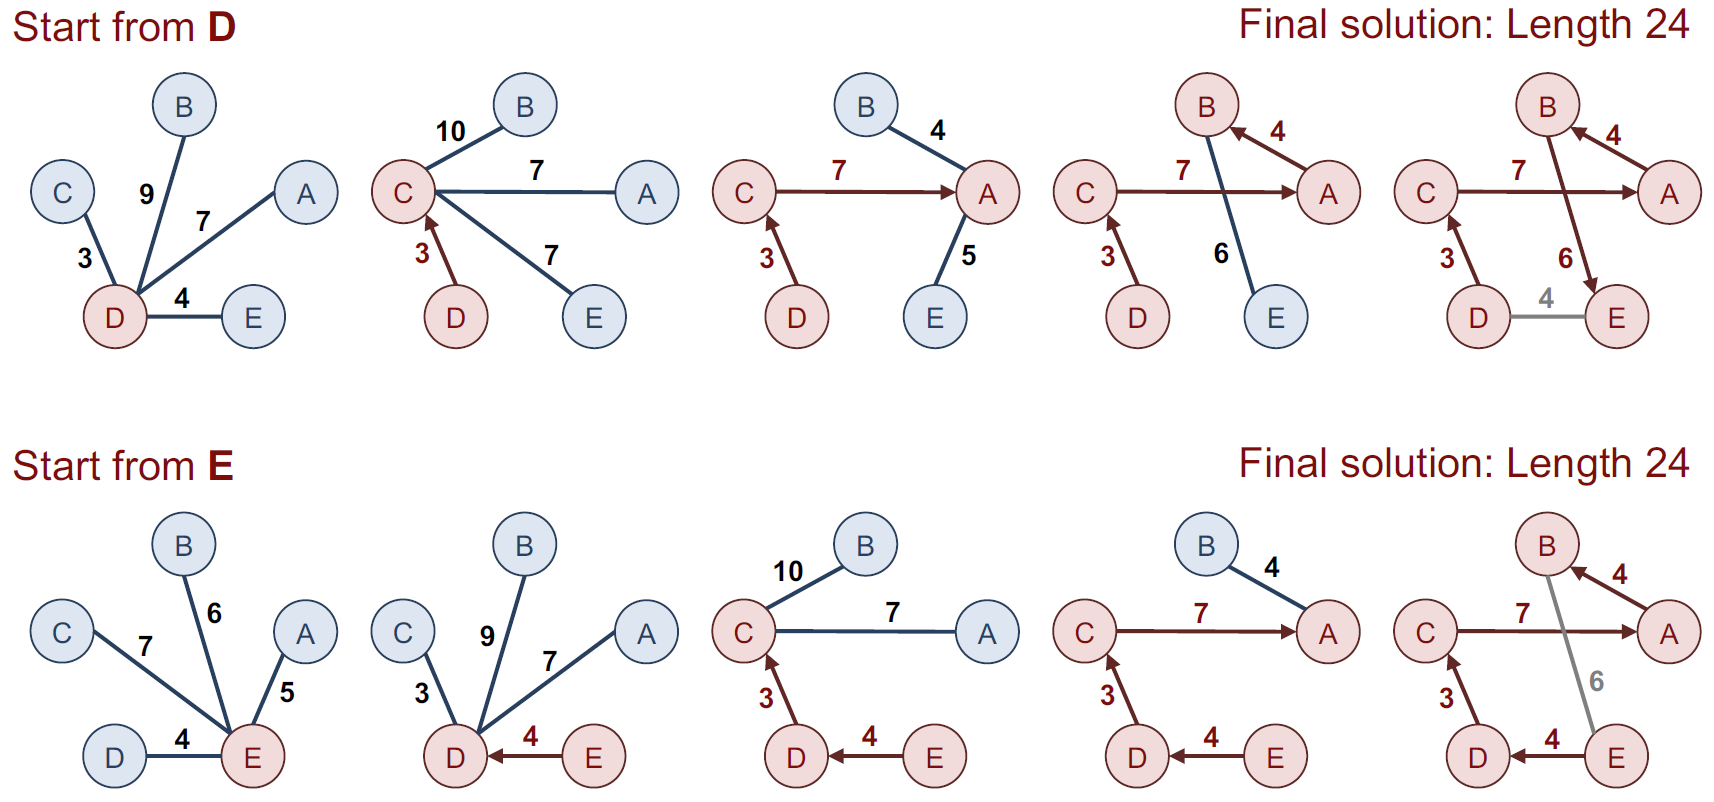
\includegraphics[width=0.85\textwidth]{img/approximation/TspGreedy3.png}\end{center}

% finished code
%\lstinputlisting[language=C++]{src/approximation/greedy.cpp}

\subsection{Local search}

The local search approach generally involves guessing a solution to the problem and then improving this solution by swapping. Applied to the TSP, this involves guessing a possible path and swapping two cities and calculating the length of the new path until the length can no longer be reduced. The central problem with the local search algorithm, however, is that it can get stuck at local minima of the problem, which can be somewhat improved with tweaks such as more complicated swapping. The algorithm proceeds as follows:

\begin{enumerate}
    \item Guess a solution.
    \item Interchange two cities and evaluate new tour $\rightarrow$ take if length decreases.
    \item Repeat this step until the length can no longer be reduced.
\end{enumerate}

\begin{center}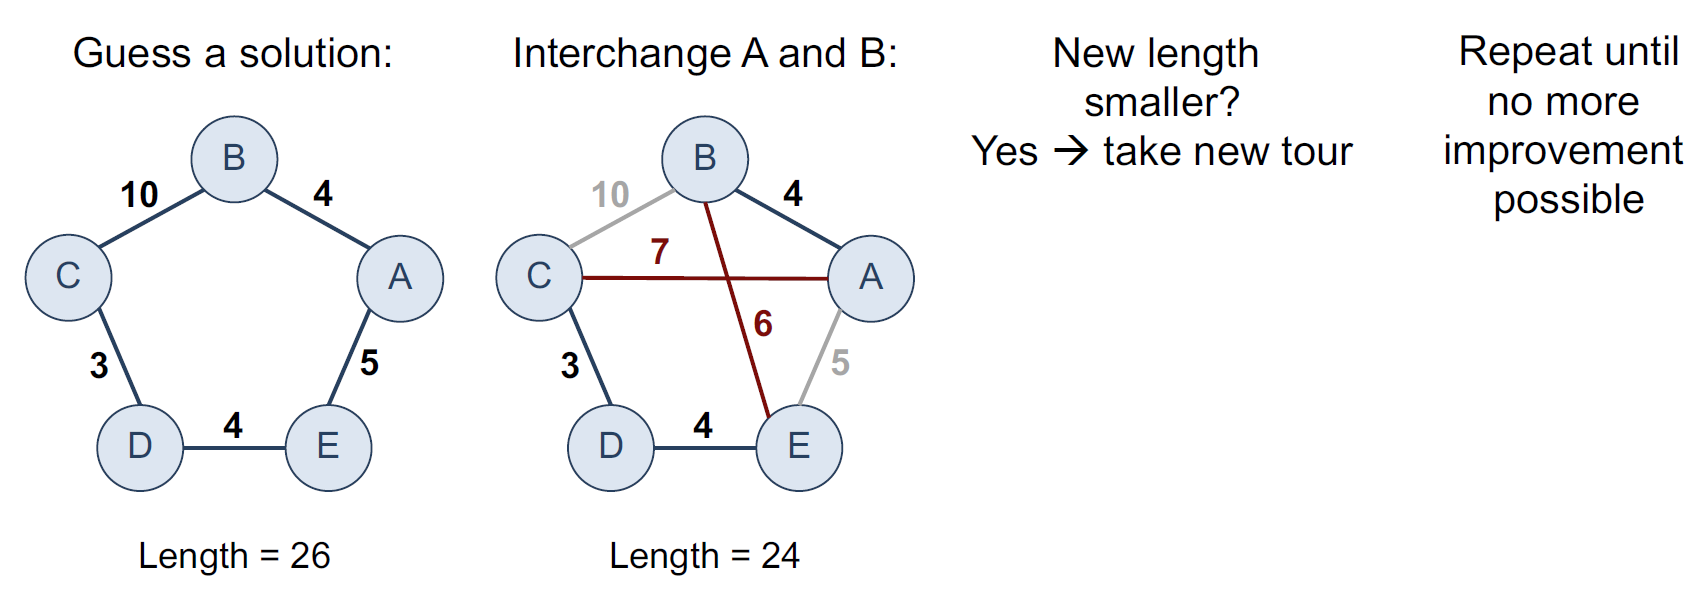
\includegraphics[width=0.85\textwidth]{img/approximation/TspLocalSearch.png}\end{center}

% not finished code
%\lstinputlisting[language=C++]{src/approximation/local_search.cpp}

